\icode{E-MD-SI-L2-261119-001}
在光滑的水平面上，有两个相互接触的物体如图所示。已知 \(M > m\)，第一次用水平力 \(F\) 由左向右推 \(M\)，物体间的相互作用力为 \(N_1\)，此时物体加速度为 \(a_1\)；第二次用同样大小的水平力 \(F\) 由右向左推 \(m\)，物体间的相互作用力为 \(N_2\)，此时物体加速度为 \(a_2\)。则\paren[]

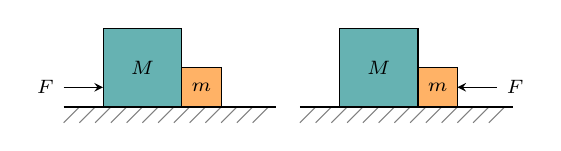
\begin{tikzpicture}[>=stealth,font=\scriptsize]
	\draw[fill=teal!60] (0,0) rectangle(1,1)node[midway]{\(M\)};
	\draw[fill=orange!60] (1,0) rectangle(1.5,.5)node[midway]{\(m\)};
	\foreach \x in {-.5,-.3,...,2}
		\draw[gray] (\x,-.2)--++(.2,.2);
	\draw[thick] (-.5,0)--(2.2,0);
	\draw[->] (-.5,.25)node[left]{\(F\)}--++(.5,0);
	\begin{scope}[xshift=3cm]
		\draw[fill=teal!60] (0,0) rectangle(1,1)node[midway]{\(M\)};
		\draw[fill=orange!60] (1,0) rectangle(1.5,.5)node[midway]{\(m\)};
		\foreach \x in {-.5,-.3,...,2}
			\draw[gray] (\x,-.2)--++(.2,.2);
		\draw[thick] (-.5,0)--(2.2,0);
		\draw[->] (2,.25)node[right]{\(F\)}--++(-.5,0);
	\end{scope}
\end{tikzpicture}
\begin{choices}
	\item \(N_1 > N_2, a_1 < a_2\)
	\item \(N_1 = N_2, a_1 = a_2\)
	\item \(N_1 < N_2, a_1 > a_2\)
	\item \(N_1 < N_2, a_1 = a_2\)
\end{choices}
\begin{answer}
	D\qquad 提示：
\end{answer}